\clearpage
\documentclass[a4paper,12pt,notitlepage]{article}

\frenchspacing
\usepackage{a4}
\usepackage[pdftitle={Vypracovane otazky ke statnicim}, pdfauthor={studenti MFF}, pdfdisplaydoctitle=true, colorlinks=false,unicode=true,pdfborder=0 0 0]{hyperref}
\usepackage{czech}
\usepackage{ucs}
\usepackage[utf8x]{inputenc}

\title{Vypracovane otazky ke statnicim}
\author{studenti MFF}

\usepackage{graphicx}
\usepackage{amsmath,amssymb,amsthm}
\usepackage{color}
\usepackage[left=3cm, right=3cm, top=3cm, bottom=3cm]{geometry} % nastavení dané velikosti okrajů

\usepackage{float}
\newfloat{kod}{h}{kod}
\floatname{kod}{Kód}

%Vacsina prostredi je dvojjazicne. V pripade, ze znenie napr pozorovania je pisane po slovensky, malo by byt po slovensky aj oznacenie.

\newenvironment{pozadavky}{\pagebreak[2]\noindent\textbf{Požadavky}\par\noindent\leftskip 10pt}{\par\bigskip}
\newenvironment{poziadavky}{\pagebreak[2]\noindent\textbf{Požiadavky}\par\noindent\leftskip 10pt}{\par\bigskip}

\newenvironment{definice}{\pagebreak[2]\noindent\textbf{Definice}\par\noindent\leftskip 10pt}{\par\bigskip}
\newenvironment{definiceN}[1]{\pagebreak[2]\noindent\textbf{Definice~}\emph{(#1)}\par\noindent\leftskip 10pt}{\par\bigskip}
\newenvironment{definicia}{\pagebreak[2]\noindent\textbf{Definícia}\par \noindent\leftskip 10pt}{\par\bigskip}
\newenvironment{definiciaN}[1]{\pagebreak[2]\noindent\textbf{Definícia~}\emph{(#1)}\par\noindent\leftskip 10pt}{\par\bigskip}

\newenvironment{pozorovani}{\pagebreak[2]\noindent\textbf{Pozorování}\par\noindent\leftskip 10pt}{\par\bigskip}
\newenvironment{pozorovanie}{\pagebreak[2]\noindent\textbf{Pozorovanie}\par\noindent\leftskip 10pt}{\par\bigskip}
\newenvironment{poznamka}{\pagebreak[2]\noindent\textbf{Poznámka}\par\noindent\leftskip 10pt}{\par\bigskip}
\newenvironment{poznamkaN}[1]{\pagebreak[2]\noindent\textbf{Poznámka~}\emph{(#1)}\par\noindent\leftskip 10pt}{\par\bigskip}
\newenvironment{lemma}{\pagebreak[2]\noindent\textbf{Lemma}\par\noindent\leftskip 10pt}{\par\bigskip}
\newenvironment{lemmaN}[1]{\pagebreak[2]\noindent\textbf{Lemma~}\emph{(#1)}\par\noindent\leftskip 10pt}{\par\bigskip}
\newenvironment{veta}{\pagebreak[2]\noindent\textbf{Věta}\par\noindent\leftskip 10pt}{\par\bigskip}
\newenvironment{vetaN}[1]{\pagebreak[2]\noindent\textbf{Věta~}\emph{(#1)}\par\noindent\leftskip 10pt}{\par\bigskip}
\newenvironment{vetaSK}{\pagebreak[2]\noindent\textbf{Veta}\par\noindent\leftskip 10pt}{\par\bigskip}
\newenvironment{vetaSKN}[1]{\pagebreak[2]\noindent\textbf{Veta~}\emph{(#1)}\par\noindent\leftskip 10pt}{\par\bigskip}

\newenvironment{dusledek}{\pagebreak[2]\noindent\textbf{Důsledek}\par\noindent\leftskip 10pt}{\par\bigskip}
\newenvironment{dosledok}{\pagebreak[2]\noindent\textbf{Dôsledok}\par\noindent\leftskip 10pt}{\par\bigskip}

\newenvironment{dokaz}{\pagebreak[2]\noindent\leftskip 10pt\textbf{Dôkaz}\par\noindent\leftskip 10pt}{\par\bigskip}
\newenvironment{dukaz}{\pagebreak[2]\noindent\leftskip 10pt\textbf{Důkaz}\par\noindent\leftskip 10pt}{\par\bigskip}

\newenvironment{priklad}{\pagebreak[2]\noindent\textbf{Příklad}\par\noindent\leftskip 10pt}{\par\bigskip}
\newenvironment{prikladSK}{\pagebreak[2]\noindent\textbf{Príklad}\par\noindent\leftskip 10pt}{\par\bigskip}
\newenvironment{priklady}{\pagebreak[2]\noindent\textbf{Příklady}\par\noindent\leftskip 10pt}{\par\bigskip}
\newenvironment{prikladySK}{\pagebreak[2]\noindent\textbf{Príklady}\par\noindent\leftskip 10pt}{\par\bigskip}

\newenvironment{algoritmusN}[1]{\pagebreak[2]\noindent\textbf{Algoritmus~}\emph{(#1)}\par\noindent\leftskip 10pt}{\par\bigskip}
%obecne prostredie, ktore ma vyuzitie pri specialnych odstavcoch ako (uloha, algoritmus...) aby nevzniklo dalsich x prostredi
\newenvironment{obecne}[1]{\pagebreak[2]\noindent\textbf{#1}\par\noindent\leftskip 10pt}{\par\bigskip}


\newenvironment{penumerate}{
\begin{enumerate}
  \setlength{\itemsep}{1pt}
  \setlength{\parskip}{0pt}
  \setlength{\parsep}{0pt}
  %\setlength{\topsep}{200pt}
  \setlength{\partopsep}{200pt}
}{\end{enumerate}}

\def\pismenka{\numberedlistdepth=2} %pouzit, ked clovek chce opismenkovany zoznam...

\newenvironment{pitemize}{
\begin{itemize}
  \setlength{\itemsep}{1pt}
  \setlength{\parskip}{0pt}
  \setlength{\parsep}{0pt}
}{\end{itemize}}

\definecolor{gris}{gray}{0.95}
\newcommand{\ramcek}[2]{\begin{center}\fcolorbox{white}{gris}{\parbox{#1}{#2}}\end{center}\par}

\clearpage

\title{\LARGE Učební texty ke státní závěrečné zkoušce \\ Softwarové systémy \\ Softwarové inženýrství}


\begin{document}

\maketitle

\vspace{10mm}
\begin{center}
\includegraphics[scale=0.5]{../common/logo.pdf}
\end{center} 

\clearpage
\input{uvod.tex}
\clearpage

\tableofcontents

\input{i2/spolecne.tex}
\definecolor{orange}{RGB}{255,127,0}

\newcommand{\TODO}[1]{\colorbox{orange}{TODO: #1}}
\newcommand{\derives}[1]{\implies \hskip -0.7em ^#1 \hskip 0.7em}







\newpage
\section{Programovací jazyky a překladače}
\begin{pozadavky}
\begin{pitemize}
\item Struktura kompilátoru a navazujících nástrojů (linkery, loadery, debuggery, knihovny, preprocesory).
\item Konečné automaty a lexikální analýza.
\item Syntaktická analýza - LL, LR techniky.
\item Syntaxí řízený překlad a atributové gramatiky.
\item Reprezentace programu mezikódem.
\item Překlad výrazů a programových struktur.
\item Rozsahy platnosti proměnných, aktivační záznamy, implementace vnořených procedur, volací konvence.
\item Vliv architektury počítače na generování kódu a optimalizaci.
\item Metody generování kódu, přidělování registrů, scheduling, optimalizace.
\item Podpora kompilátorů pro synchronizační primitiva, vlákna.
\item Objektově orientované jazyky a principy jejich implementace.
\item Překladače vs. interpretry, skriptovací jazyky.
\end{pitemize}
\end{pozadavky}

\subsection{Struktura kompilátoru a navazujících nástrojů (linkery, loadery, debuggery, knihovny, preprocesory).}

\begin{figure}[h]
	\centering
	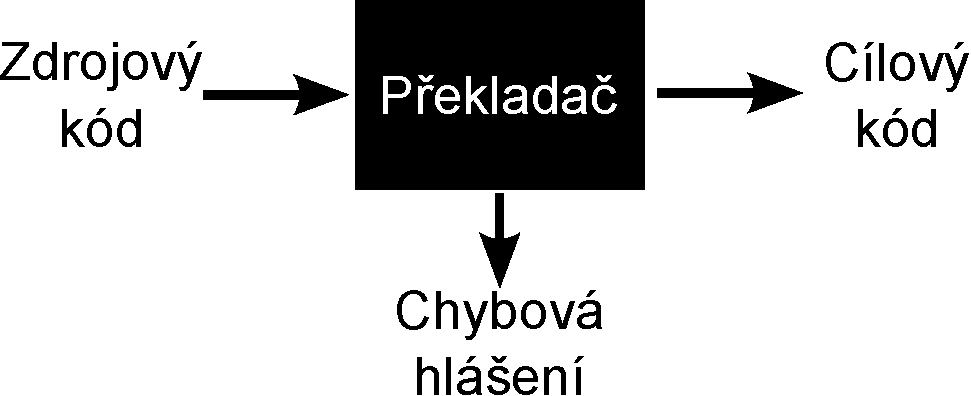
\includegraphics[width=8cm]{i2/softwarove_inzenyrstvi/obrazky/Prekladac-cerna_skrinka.pdf}
	\caption{Překladač jako černá skříňka.}
	\label{pic:Prekladac-cerna_skrinka}
\end{figure}
\begin{definiceN}{Překladač}
Mějme vstupní jazyk \(L_{in}\) generovaný gramatikou \(G_{in}\).
Dále mějme výstupní jazyk \(L_{out}\) generovaný gramatikou \(G_{out}\) nebo přijímaný automatem \(A_{out}\).
\emph{Překladač} je zobrazení \(L_{in} \to L_{out}\), kde \(\forall w_{in} \in L_{in} \exists w_{out} \in L_{out}\) a zároveň pro \(w_{in} \notin L_{in}\) zobrazení neexistuje.
\end{definiceN}


\subsubsection{Příklady užití technik překladačů}
\begin{pitemize}
	\item Zvýrazňování syntaxe v editorech,
	\item pretty-printer,
	\item statické kontroly kódu,
	\item interpretery,
	\item překladače modelovacích jazyků,
	\item dotazovací jazyky (SQL).
\end{pitemize}


\subsubsection{Historie a srovnání metod tvorby a spouštění programů}
Následující části jsou dobře rozkreslené na slajdech (od p. Bednárka) z C++.

Nejdříve (~1940) se programovalo přímo v binárním kódu, tedy přesně v tom, čemu rozuměl procesor. Později (~1950) byl vymyšlen assembler, tedy jazyk, který zcela přesně popisoval co bude procesor dělat, ale v lidsky čitelnější podobě (do podoby čitelné procesorem se dostane jak jinak než překladačem). Také se v počítačích objevil operační systém, takže se nespouštěl přímo program, ale nejprve se spustil OS a ten teprve (pomocí loaderu) načetl do paměti program a spustil jej. Program tedy už nemusel být ve formátu, kterému rozumí přímo procesor, ale mohl být obalen dalšími informacemi, které rozpoznával a zpracovával operační systém. Potom se objevily jazyky na vyšší úrovni, které se do spustitelného souboru kompilovaly a tyto jazyky byly vyšší a vyšší.

Další možností spouštění programů je jejich interpretace, tedy vlastně spojení kompilace a spouštění. Program je řádku po řádce parsován a prováděn. Běh takového programu je však pomalý, což se dá vyřešit tak, že program se nejprve (při spouštění) přeloží do mezikódu a ten je teprve interpretován (mezikód je přinejmenším menší). Překlad se ale dělá při každém spuštění, což je neefektivní. Překlad (do mezikódu) se může udělat jen jednou a vytvořit tak jakýsi soubor spustitelný pomocí interpretru. Výhodou (oproti klasickému překladu přímo do binární podoby, které rozumí CPU) je platformní nezávislost mezikódu. Stačí aby pro daný procesor existoval interpret a je možné mezikód na tomto procesoru spustit. Opět se však potýkáme s neefektivitou interpretace mezikódu. Jako řešení byl vymyšlen tzv. JIT (Just in time compiler), který mezikód za běhu programu překládá do strojového kódu a ten teprve spouští. Výhodou je, že pokud se nějaká část programu provádí znovu, tak ji stačí jen spustit a už není potřeba mezikód.

Poznámka: Dnešní překladače již většinou vygenerují optimálnější kód než by člověk dokázal napsat.

\begin{table}[h]
	{\centering
	\begin{tabular}{ l || p{4cm} | p{4cm} }
		& JIT & Klasika \\
		\hline
		\hline
		Distribuce & bytecode & binární instrukce \\
		\hline
		Závislost distribuce & jazyk a překladač & procesor a OS \\
		\hline
		Výhoda překladače & překladač zná přesně cílový procesor, může sledovat chování programu & překladač má hodně času na překlad
	\end{tabular} \\
	}
	\caption{Srovnání klasické metody kompilace a JIT}
	\label{tab:Srovnani_JIT}
\end{table}


\subsubsection{Klasická kompilace}
\begin{figure}[h]
	\centering
	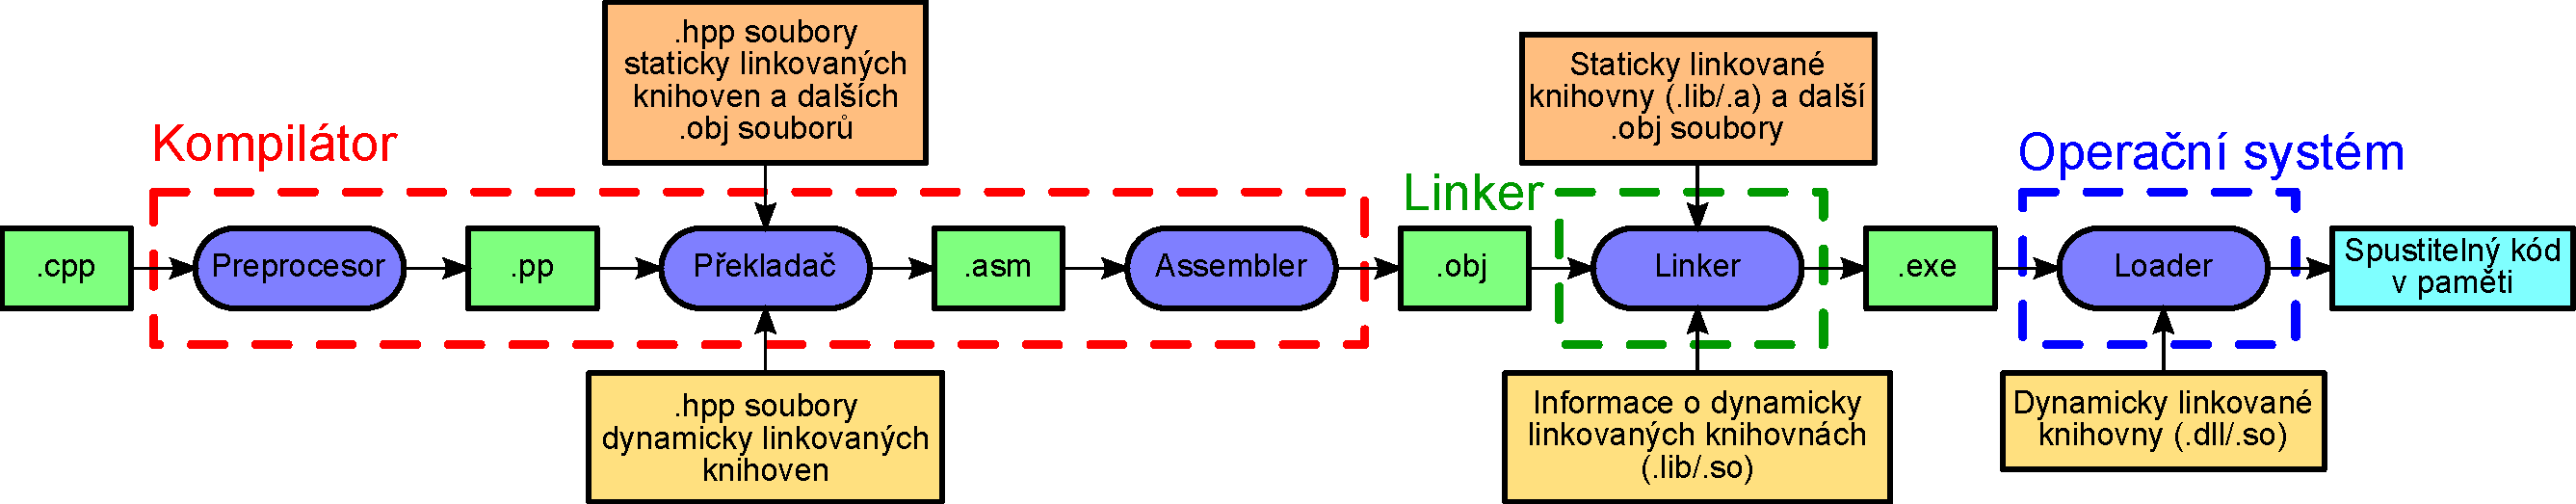
\includegraphics[width=15cm]{i2/softwarove_inzenyrstvi/obrazky/Preklad.pdf}
	\caption{Průběh překladu zdrojových kódů v C++.}
	\label{pic:Preklad}
\end{figure}

Všimněte si, že to, co se běžně nazývá překladačem je vlastně složeno z několika menších překladačů (preprocesor, překladač, assembler).

\paragraph{Překladač}
Na obrázku \ref{pic:Preklad} je červeně vyznačena oblast, kterou má na starosti program, který je běžně označován jako \emph{překladač} či \emph{kompilátor}. Tento program tedy provádí překlad ze zdrojových kódů do binárních souborů (za pomoci hlavičkových souborů). Tento program poběží tolikrát, kolik je v kompilovaném projektu kódu (.cpp). Pokud je v souboru .cpp odkaz na něco (proměnnou, funkci aj.) z jiného .cpp nebo z knihovny, tak na daném místě překladač nechá volné místo pro doplnění adresy (musí vědět kolik místa nechat -- proto potřebuje hlavičkové soubory odkazovaných souborů a knihoven).

\paragraph{Linker}
Jednotlivé soubory .obj, které vytvoří překladač je ještě potřeba spojit do jednoho spustitelného souboru. To má na starosti tzv. linker, který je spojí a doplní adresy do prázdných míst, které tam nechal překladač. Nemůže však vyplnit místa pro dynamicky linkované knihovny, proto je opět nechá prázdná.

\paragraph{Loader}
Hlavním úkolem loaderu je načíst program do paměti a spustit ho. Před jeho spuštěním je však potřeba přilinkovat ještě dynamicky linkované knihovny, takže loader vyplní prázdná místa, která mu tam nechal linker. Dynamické linkování se dá dělat několika způsoby. Buď se vyplní rovnou všechny adresy na všech místech, kde se program odkazuje do knihovny (těch ale může být hodně), nebo se do knihovny neadresuje přímo, ale přičítá se její offset a loader vyplní jen tento offset. Druhá možnost má nevýhodu v tom, že při každém volání se musí zjistit offset a ten se ještě musí přičíst k adrese v knihovně. Dá se tedy udělat kompromis, totiž že se udělá tabulka (používaných) adres v knihovně, kterou loader vyplní. V tabulce nejsou duplicity, takže vyplnění nebude trvat tak dlouho a při volání se nemusí nic sčítat, pouze se provede dereference. Která možnost se použije samozřejmě nemůže rozhodovat sám loader (potřebuje aby mu vhodné struktury připravil už překladač).

\paragraph{Debugger}
K ladění programů slouží debugger, který používá jak zkompilovaný program, tak zdrojové kódy. Potřebuje se však nějak dozvědět, která část zkompilovaného programu odpovídá které části zdrojových kódů. Tuto informaci mu poskytuje překladač.

\paragraph{Knihovny}
Knihovny se dělí na statické a dynamické. Statické knihovny se linkují s programem za kompilace (linkerem) a dynamické se linkují před spuštěním (loaderem). Způsoby linkování dynamických knihoven viz část o loaderu. Dynamické knihovny lze navíc načítat až za běhu aplikace. Knihovna tak může být načtena do paměti až v případě potřeby.

\paragraph{Preprocesor}
Zvláštní částí kompilátoru je preprocesor, což je vlastně sám překladač. Překládá totiž kód z jazyka preprocesoru do jazyka C/C++/... Z možností preprocesoru jazyka C se nejčastěji používá podmíněný překlad, jehož použití je vidět na ukázce kódu \ref{cod:Preprocesor}. V jazyce C se preprocesor používal více (např. pro konstanty), v C++ již byly některá tato použití nahrazena možnostmi samotného jazyka C++.
\begin{kod}[h]
	\begin{verbatim}
		#ifdef unix
		  std::cout << "Ahoj unixáku!";
		#else
		  std::cout << "Ahoj neunixáku!";
		#endif
	\end{verbatim}
	\caption{Příklad použití preprocesoru.}
	\label{cod:Preprocesor}
\end{kod}


\subsubsection{Struktura překladače}
\begin{figure}[h]
	\centering
	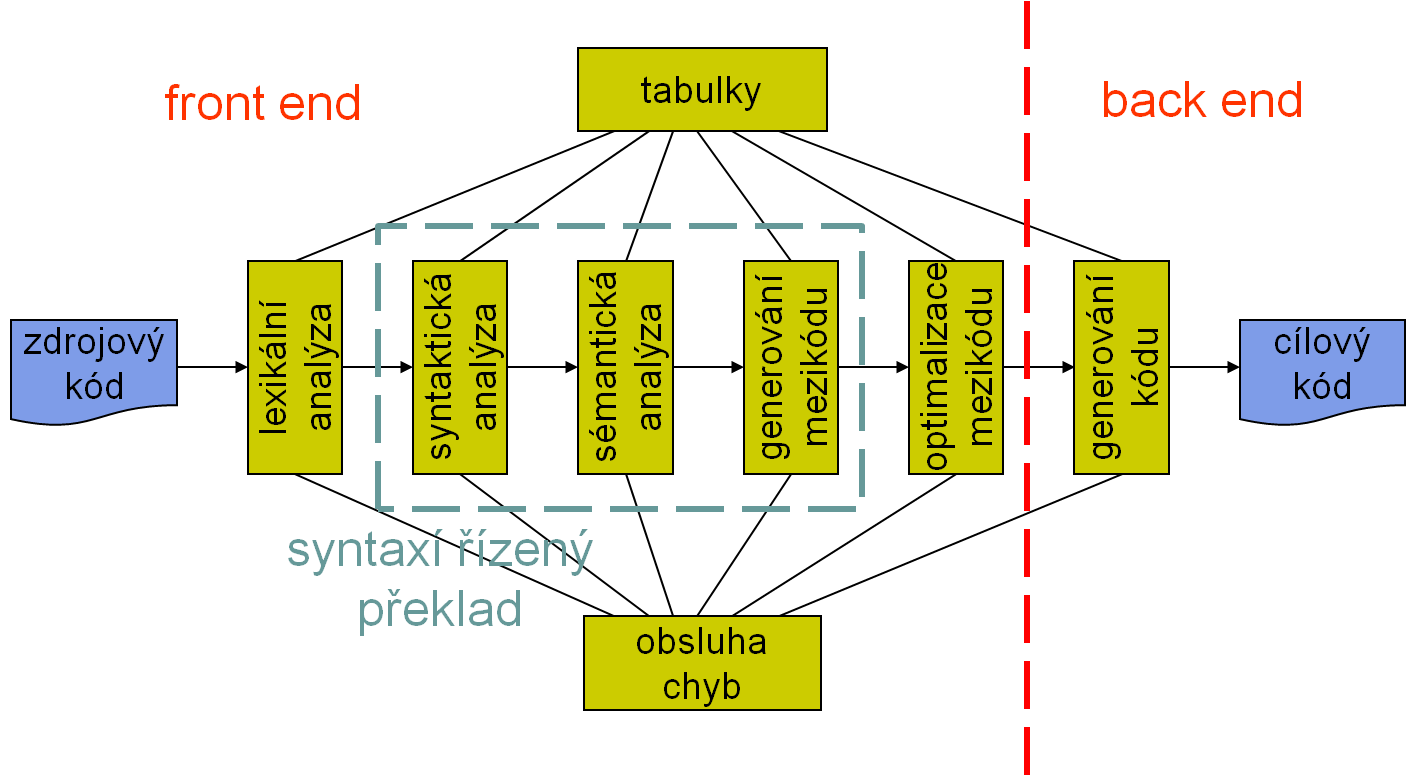
\includegraphics[width=15cm]{i2/softwarove_inzenyrstvi/obrazky/Faze_prekladu.png}
	\caption{Fáze překladu.}
	\label{pic:Faze_prekladu}
\end{figure}
Překladač se skládá z front endu a back endu. Překlad probíhá v několika fázích. Budeme předpokládat syntaxí řízený překlad. Překlad začíná spuštěním syntaktického analyzátoru, který postupně žádá lexikální analyzátor o další token. Ze získaných tokenů se snaží \uv{složit} některé z pravidel gramatiky (buď shora dolů nebo naopak). Jakmile jej najde, proběhne sémantická analýza, která podle pravidla upraví tabulky symbolů a případně proběhne generování mezikódu. Jakmile je dokončeno generování mezikódu, mohou na něm proběhnout optimalizace. Mezikód se potom předá back endu, který z něj vygeneruje kód na kterém může opět provést další (platformě specifické) optimalizace. Pokud se během celého procesu objeví chyba, překladač by se ji měl pokusit nějakým způsobem ignorovat (ale nahlásit) a pokračovat dál pokud možno tak, aby tím nevznikly další domnělé chyby a zároveň aby se na žádnou chybu nezapomnělo.




\subsection{Konečné automaty a lexikální analýza.}

\TODO{Dopsat tuto otázku: Co mají konečné automaty společného s lexikální analýzou?}




\subsection{Syntaktická analýza - LL, LR techniky.}

\begin{figure}[h]
	\centering
	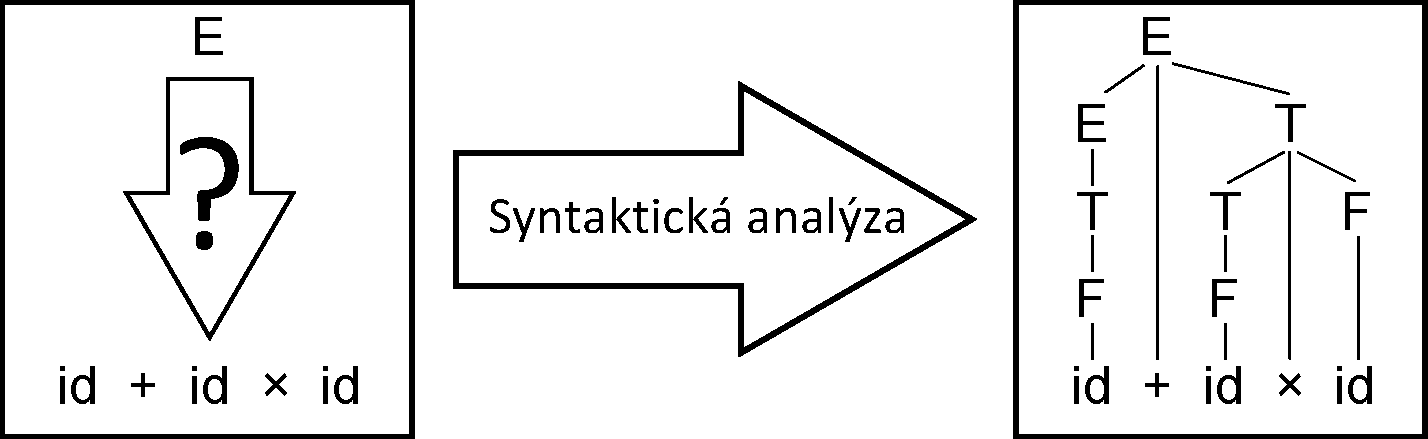
\includegraphics[width=8cm]{i2/softwarove_inzenyrstvi/obrazky/Syntakticka_analyza.pdf}
	\caption{Hlavní úkol syntaktické analýzy.}
	\label{pic:Syntakticka_analyza}
\end{figure}

Hlavním úkolem syntaktické analýzy je rozpoznat, jestli slovo (=zdrojový kód) na vstupu je slovem ze vstupního jazyka (=korektním programem v daném jazyce) a vyrobí jeho derivační strom.

Používá-li se technika syntaxí řízeného překladu, syntaktická analýza řídí celý překladač (rozuměj hlavní cyklus překladače je v syntaktickém analyzátoru).

\begin{figure}[h]
	\centering
	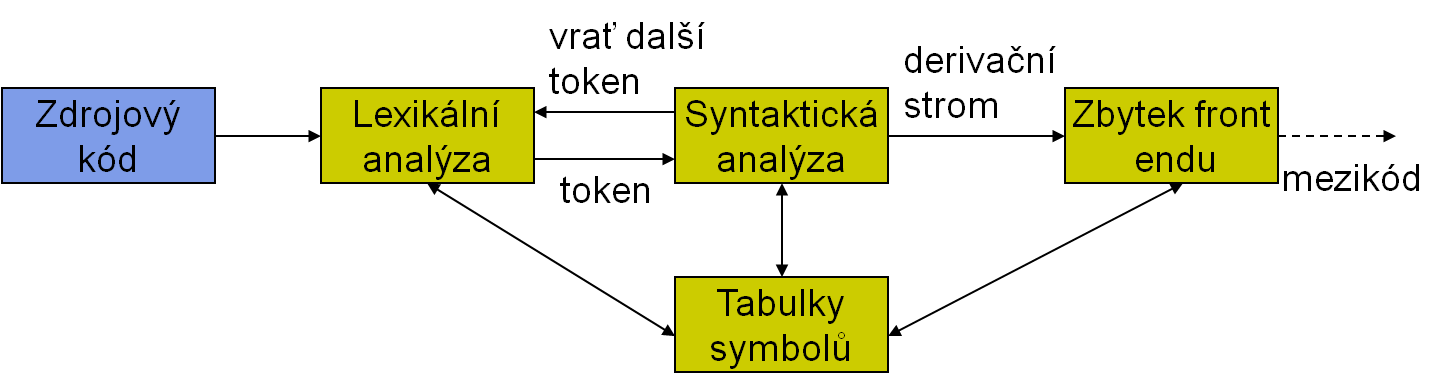
\includegraphics[width=13cm]{i2/softwarove_inzenyrstvi/obrazky/Syntakticka_analyza_v_prekladaci.png}
	\caption{Syntaktická analýza ve vztahu k ostatním částem překladače.}
	\label{pic:Syntakticka_analyza_v_prekladaci}
\end{figure}

Na obrázku \ref{pic:Syntakticka_analyza_v_prekladaci} je vidět propojení mezi syntaktickou analýzou a tabulkou symbolů, které by správně nemělo být potřeba, ale využívá se k obejití některých kontextových vlastností jazyka.

Je-li řeč o bezkontextových gramatikách, což běžné jazyky (přibližně) splňují, je potřeba zásobníkový automat, který postaví derivační strom. Vlastnosti jazyka, které přesahují bezkontextovost (např. deklarace identifikátoru před použitím nebo stejný počet parametrů v deklaraci a volání funkce) jsou potom řešeny při sémantické analýze.

\begin{definice}
	Znak nazveme \emph{symbolem}, je-li tento znak terminálem nebo neterminálem.
\end{definice}


\subsubsection{Jednoznačnost gramatiky}

Ke každému slovu musí být derivační strom určen jednoznačně. Případem situace, kdy tomu tak nemusí být a je třeba gramatiku upravit (oproti přirozené verzi), je problém \uv{dangling else}, kdy podle (přirozené) gramatiky nevíme, ke kterému \uv{ifu} větev else patří.

\begin{kod}[h]
	\begin{verbatim}
		stmt -> if expr then stmt
		      | if expr then stmt else stmt
		      | while expr do stmt
		      | goto num
	\end{verbatim}
	\caption{Původní (přirozená) gramatika.}
	\label{cod:Prirozena_gramatika}
\end{kod}

\begin{kod}[h]
	\begin{verbatim}
		stmt -> hodny_stmt
		      | zly_stmt
		hodny_stmt -> if expr then hodny_stmt else hodny_stmt
		      | while expr do hodny_stmt
		      | goto num
		zly_stmt -> if expr then zly_stmt
		      | if expr then hodny_stmt else zly_stmt
		      | while expr do lzy_stmt
	\end{verbatim}
	\caption{Jednoznačná gramatika.}
	\label{cod:Jednoznacna_gramatika}
\end{kod}

V ukázkách kódu \ref{cod:Prirozena_gramatika} a \ref{cod:Jednoznacna_gramatika} \uv{while} reprezentuje všechny příkazy, které mají na konci \uv{stmt} a \uv{goto} reprezentuje všechny příkazy, které na konci \uv{stmt} nemají.


\subsubsection{Levá rekurze}

Dalším problémem pro syntaktickou analýzu, pokud dělá analýzu shora dolů, je levá rekurze.

\begin{definice}
	Řekneme, že gramatika je \emph{levě rekurzivní}, pokud obsahuje neterminál \(A\), pro který platí, \(A \derives{+} A \alpha\), kde \(\alpha\) je nějaký řetězec symbolů. Tedy \(A\) se dá pomocí pravidel gramatiky převést na \(A\alpha\). Příklad odstranění levé rekurze je vidět na ukázce kódu \ref{cod:Odstraneni_rekurze}.
\end{definice}

\begin{kod}[h]
	Původní gramatika
	\begin{verbatim}
		A -> Aa
		A -> b
	\end{verbatim}
	
	Nová gramatika
	\begin{verbatim}
		A -> bB
		B -> aB
		B -> {lambda}
	\end{verbatim}
	\caption{Odstranění levé rekurze.}
	\label{cod:Odstraneni_rekurze}
\end{kod}


\subsubsection{Levá faktorizace}

V gramatice se může objevit také tzv. levá faktorizace, což je situace, kdy máme k dispozici dvě pravidla, ale podle prvního neterminálu si nedokážeme vybrat, které použít. Řešení je jednoduché: Vytvořit nové pravidlo, které bude obsahovat začátek a teprve v místě kde se původní pravidla lišila bude další neterminál. Konkrétní řešení ukazuje kód \ref{cod:Odstraneni_faktorizace}.

\begin{kod}[h]
	Původní gramatika
	\begin{verbatim}
		A -> ab
		A -> ac
	\end{verbatim}
	
	Nová gramatika
	\begin{verbatim}
		A -> aB
		B -> b
		B -> c
	\end{verbatim}
	\caption{Odstranění levé faktorizace.}
	\label{cod:Odstraneni_faktorizace}
\end{kod}


\subsubsection{Postup syntaktické analýzy}

Syntaktická analýza může probíhat dvěma směry, a to buď shora dolů nebo zdola nahoru.

\paragraph{Shora dolů} Při analýza shora dolů se analyzátor snaží určit použitá pravidla v derivačním stromě od jeho kořene. Tento postup lze realizovat buď rekurzivním sestupem (obvyklejší) nebo pomocí LL automatu. Analýza shora dolů najde nejlevější derivaci. Tento postup se používá např. v generátoru parserů ANTLR.

\paragraph{Zdola nahoru} Naopak analýza zdola nahoru se snaží hledat použitá pravidla zdola nahoru, tedy derivační strom vytváří tak, že postupně listy spojuje do menších stromů a ty do větších až dostane celý derivační strom. Tento postup lze realizovat LR automatem. Analýza zdola nahoru hledá nejpravější derivaci (ale pozpátku).Tento postup se používá např. v generátoru parserů Bison (Bison generuje ve výchozím nastavení parsery rozpoznávající jen \(LALR(1)\) -- aby byly parsery jednodušší/rychlejší). Oproti postupu shora dolů má postup zdola nahoru tyto výhody:

\begin{pitemize}
	\item Lze rozpoznávat všechny programovací jazyky zapsané bezkontextovou gramatikou.
	\item Dá se implementovat stejně efektivně jako metoda shora dolů.
	\item Třída rozpoznávaných jazyků \(LR(1)\) je vlastní nadmnožinou třídy \(LL(1)\).
\end{pitemize}

\subsubsection{Typy gramatik}

Gramatiky související s překladači se označují kombinací, která odpovídá vzoru \(PXY(k)\), kde

\begin{pitemize}
	\item \(X \in \{L, R\}\) označuje směr čtení vstupu (v našem případě vždy \(L\),
	\item \(Y \in \{L, R\}\) označuje druh derivace, tedy \(L\) odpovídá levé derivaci a \(R\) odpovídá pravé derivaci.
	\item \(P\) označuje prefix, který nemá jednotný význam, ale dají se pomocí něj gramatiky členit ještě jemněji.
	\item \(k \in \mathbb{N}\) označuje výhled automatu, tedy počet symbolů (tokenů), podle kterých se může automat rozhodovat, které vybrat pravidlo. Obvykle \(k = 1\), ale může být i \(k = 0\).
\end{pitemize}

Příklady: \(LL(1)\), \(LR(0)\), \(LR(1)\), \(LL(k)\), \(SLR(1)\), \(LALR(1)\).

\vskip 1em
\begin{definiceN}{\(LL(1)\) gramatika}
	Bezkontextová gramatika \(G = (T, N, S, P)\) je \emph{\(LL(1)\) gramatika}, pokud pro každá 2 pravidla \(A \to \alpha, A \to \beta \in P\), kde \(\alpha \neq \beta\), a každé 2 levé větné formy \(uA \gamma, vA \delta\), kde \(u, v \in T^*\) a \(\gamma, \delta \in (T \cup N)^*\), platí \(FIRST(\alpha \gamma) \cap FIRST(\beta \delta) = \emptyset\).
\end{definiceN}

Tato definice se snaží říct, že pravidla jsou taková, abych podle prvního znaku jednoznačně poznal, které pravidlo mám použít (snáze se to pochopí, když člověk ví, jak funguje rekurzivní sestup a LL automat, jejichž popisy následují dále). \(\gamma\) a \(\delta\) jsou v definici aby rozhodly, pokud \(\alpha\) nebo \(\beta\) budou prázdné řetězce.

\vskip 1em
\begin{definiceN}{silná a slabá \(LL(k)\) gramatika}
	Bezkontextová gramatika \(G = (T, N, S, P)\) je \emph{silná \(LL(k)\) gramatika} pro \(k \ge 1\), pokud pro každá 2 pravidla \(A \to \alpha, A \to \beta \in P\), kde \(\alpha \neq \beta\), a každé 2 levé větné formy \(uA \gamma, vA \delta\), kde \(u, v \in T^*\) a \(\gamma, \delta \in (T \cup N)^*\), platí \(FIRST_k(\alpha \gamma) \cap FIRST_k(\beta \delta) = \emptyset\). Gramatiku nazveme \emph{slabou \(LL(k)\) gramatikou}, je-li silnou \(LL(k)\) gramatikou a navíc \(u = v\) a \(\gamma = \delta\).
\end{definiceN}

\begin{definiceN}{\(LR(k)\) gramatika}
	Bezkontextová gramatika \(G = (T, N, S, P)\) je \emph{\(LR(k)\) gramatika} pro \(k \ge 1\), pokud pro každá 2 pravidla \(A \to \alpha, A \to \beta \in P\), kde \(\alpha \neq \beta\), a každé 2 pravé větné formy \(\gamma A u, \delta A v\), kde \(u, v \in T^*\) a \(\gamma, \delta \in (T \cup N)^*\), platí \(FIRST_k(u) \cap FIRST_k(v) = \emptyset\).
\end{definiceN}

Oproti \(LL(k)\) gramatice jsou množiny \(FIRST_k\) mnohem menší a proto je větší šance, že bude průnik prázdný a proto do \(LR(k)\) patří více gramatik/jazyků.

\begin{figure}[h]
	\centering
	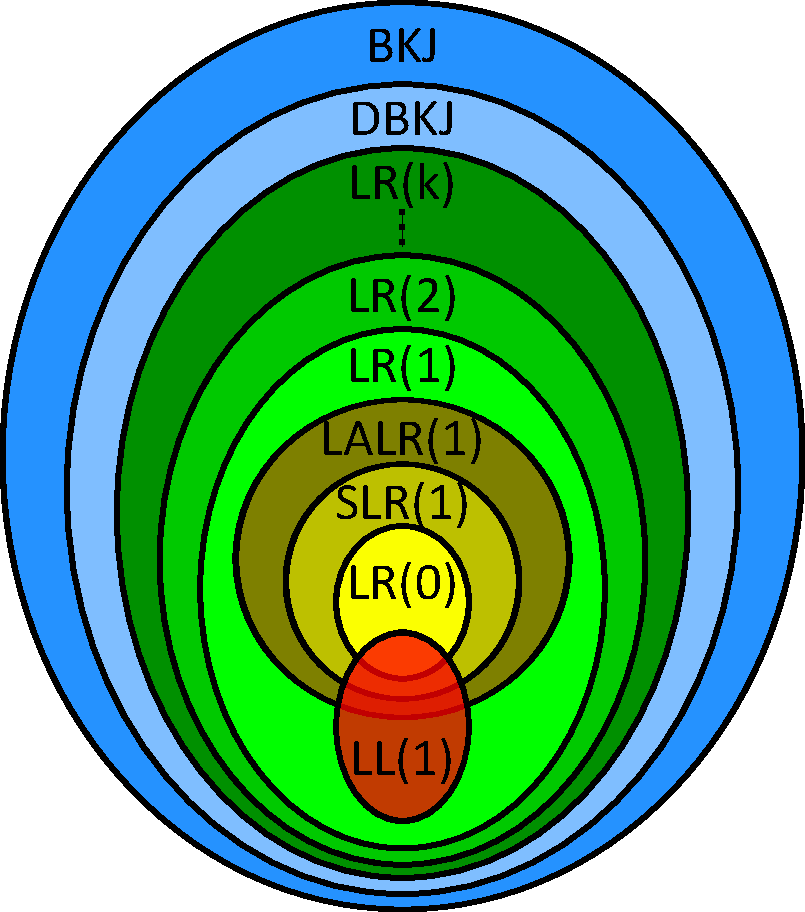
\includegraphics[width=6cm]{i2/softwarove_inzenyrstvi/obrazky/Tridy_jazyku.pdf}
	\caption{Inkluze tříd jazyků.}
	\label{pic:Tridy_jazyku}
\end{figure}

Obrázek \ref{pic:Tridy_jazyku} znázorňuje inkluzi tříd jazyků. Navíc platí, že sjednocení všech \(LR(k)\) tříd je \(DBKJ\). Přesto se jazyky nad \(LR(1)\) v praxi nepoužívají.


\subsubsection{FIRST a FOLLOW}

\begin{definiceN}{FIRST}
	Nechť \(\alpha\) je řetězec symbolů gramatiky, pak \(FIRST(\alpha)\) je množina terminálů, kterými začínají všechny řetězce derivované z \(\alpha\). Pokud \(\alpha\) může derivovat na \(\lambda\), pak je \(\lambda\) také ve \(FIRST(\alpha)\).
\end{definiceN}

\begin{definiceN}{FOLLOW}
	Nechť \(A\) je neterminál, potom \(FOLLOW(A)\) definujeme jako množinu terminálů, které se mohou vyskytovat těsně za \(A\) v nějakém řetězci, který vznikl derivací z počátečního neterminálu gramatiky (\(S \derives{*} \alpha A a \beta\), pro nějaké řetězce symbolů \(\alpha\) a \(\beta\)). Pokud je \(A\) nejpravější symbol v nějakém přepisu, pak je ve \(FOLLOW(A)\) i \(\$\) -- speciální symbol pro konec řetězce.
\end{definiceN}

\begin{priklad}
	Mějme řetězec \(ABC\), kde \(A\), \(B\) i \(C\) jsou neterminály a k tomuto řetězci jsme se dostali pravidlem \(S \to ABC\), které je jediné pro přepis \(S\). Množina \(FIRST(B)\) nám teď říká, jaké neterminály se můžou objevit na začátku řetězce, na který se přepíše neterminál \(B\). Dokonce ve \(FIRST(B)\) jsou i terminály se kterými řetězec v gramatice nemůže skončit. \(FOLLOW(B)\) nám říká, jaké terminály mohou následovat těsně za řetězcem na který se přepíše \(B\). Pokud je použité pravidlo jediné ve kterém se vyskytuje na pravé straně neterminál \(B\), pak \(FOLLOW(B) = FIRST(C)\) (až na \(\lambda\) a \(\$\)).
\end{priklad}

\paragraph{Konstrukce FIRST} Nechť \(X\) je symbol gramatiky pro který hledáme množinu \(FIRST(X)\). Je-li \(X\) terminál, pak \(FIRST(X) = \{X\}\). Existuje-li přepisovací pravidlo \(X \to \lambda\), pak přidej \(\lambda\) do \(FIRST(X)\). Pokud je \(X\) neterminál a \(X \to Y_1 Y_2 \ldots Y_k\) je přepisovací pravidlo, pak přidej \(a\) do \(FIRST(X)\) pro všechna \(a \in FIRST(Y_i)\) kde pro \(i\) platí: \(\forall j<i: \lambda \in FIRST(Y_j)\). Pokud navíc platí že \(\forall j: \lambda \in FIRST(Y_j)\), pak přidej \(\lambda\) do \(FIRST(X)\).

Množina \(FIRST\) pro řetězce symbolů se konstruuje analogicky.

\paragraph{Konstrukce FOLLOW} Nechť \(X\) je neterminál gramatiky pro který hledáme množinu \(FOLLOW(X)\). Je-li \(X\) počáteční neterminál gramatiky, přidej \(\$\) do \(FOLLOW(X)\), kde \(\$\) se speciální symbol pro konec řetězce. Existuje-li přepisovací pravidlo \(A \to \alpha X \beta\), kde \(A\) je neterminál a \(\alpha\) a \(\beta\) řetězce symbolů, pak přidej obsah množiny \(FIRST(\beta)\) kromě \(\lambda\) do \(FOLLOW(X)\). Existuje-li pravidlo \(A \to \alpha X\) nebo pravidlo \(A \to \alpha X \beta\) kde \(\lambda \in FIRST(\beta)\), pak přidej celý obsah množiny \(FOLLOW(A)\) do množiny \(FOLLOW(X)\).


\subsubsection{Rekurzivní sestup}

Pro každý neterminál existuje jedna procedura, která dělá dvě věci.
\begin{penumerate}
	\item Rozhoduje se, které pravidlo bude použito na základě výhledu (jazyk přijímaný těmito automaty je takový, že se dokáže jednoznačně rozhodnout -- mj. díky levé faktorizaci). Pravidlo s pravou stranou \(\alpha\) bude použito, pokud je výhled ve \(FIRST(\alpha)\). Existuje-li pro nějaký výhled více pravých stran, pak takovou gramatiku nelze použít pro rekurzivní sestup. Pravidlo s \(\lambda\) na pravé straně se použije tehdy, pokud výhled není ve \(FIRST\) žádné pravé strany.
	\item Kód procedury postupuje podle pravé strany vybraného pravidla, tedy pro terminály zkontroluje, jestli je terminál i na vstupu, pokud není, nastala chyba. Pro neterminál zavolá jeho proceduru.
\end{penumerate}


\subsubsection{LL automat}

\begin{figure}[h]
	\centering
	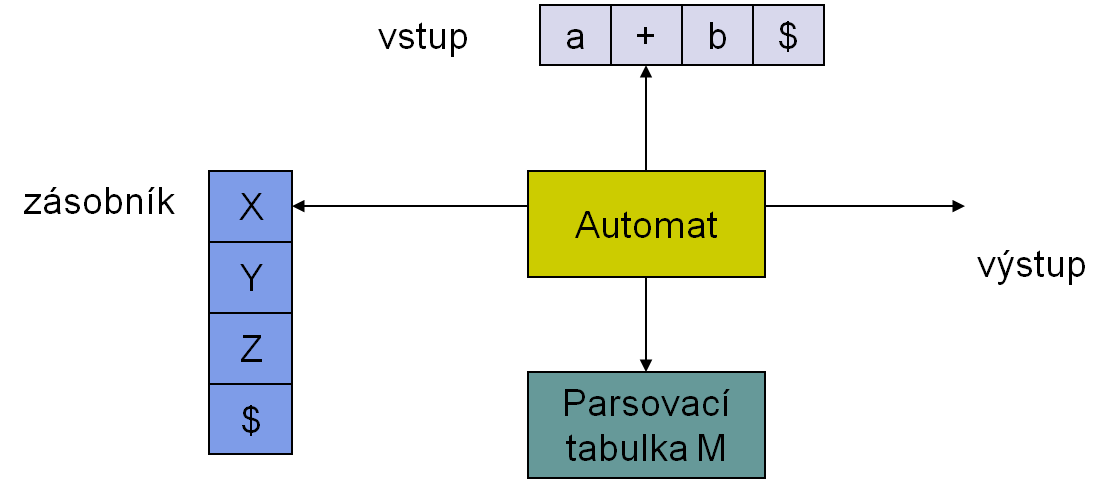
\includegraphics[width=13cm]{i2/softwarove_inzenyrstvi/obrazky/LL_automat.png}
	\caption{LL automat.}
	\label{pic:LL_automat}
\end{figure}

Na obrázku \ref{pic:LL_automat} je vidět vstup, tedy zdrojový kód, který analyzujeme. Na každém políčku je jeden symbol gramatiky, tedy tokeny, které syntaktickému analyzátoru předává lexikální analyzátor. Na zásobník se ukládají symboly, které určují co očekáváme na vstupu. Parsovací tabulka \(M\) je tabulka, ve které se indexuje pomocí neterminálu a terminálu (místo terminálu může být použit i speciální symbol \(\$\)) a v každé buňce tabulky je uloženo nejvýše jedno pravidlo gramatiky. Indexaci v tabulce budeme zapisovat jako \(M[A, a]\), kde \(A\) je neterminál a \(a\) je terminál.

\paragraph{Funkce LL automatu} Na začátku je hlava nastavena na začátek vstupu a na zásobníku je speciální symbol pro konec řetězce \(\$\) a počáteční neterminál gramatiky. V každém kroku se automat rozhoduje podle symbolu \(X\) na vrcholu zásobníku a terminálu \(a\), který je na vstupu (tedy je na něj nastavena hlava). Mohou nastat následující situace.

\begin{pitemize}
	\item Je-li \(X = a = \$\), pak se automat s úspěchem zastaví.
	\item Je-li \(X = a \neq \$\), pak se \(X\) odebere ze zásobníku a hlava se přesune o jedno políčko vstupu dál.
	\item Je-li \(X\) neterminál, pak se automat rozhodne podle \(M[X, a]\). Obsahuje-li buňka pravidlo (označme \(p\), pak se odebere \(X\) ze zásobníku a na zásobník se vloží pravá strana pravidla \(p\) tak, aby nejlevější symbol pravidla byl na vrcholu zásobníku. Zároveň je vygenerován výstup (kousek levé derivace), tedy informace o tom, že bylo použito pravidlo \(p\). Pokud buňka tabulky neobsahovala pravidlo, nahlásí se chyba.
\end{pitemize}

\paragraph{Konstrukce tabulky automatu} Teď je ještě potřeba vědět, jak zkonstruovat tabulku \(M\). Nejprve inicializujeme buňky tabulky na prázdné a potom pro každé pravidlo gramatiky \(A \to \alpha\) provedeme:

\begin{penumerate}
	\item \(\forall a \in FIRST(\alpha)\) přidáme \(A \to \alpha\) do \(M[A, a]\).
	\item Pokud \(\lambda \in FIRST(\alpha)\), pak přidáme \(A \to \alpha\) do \(M[A, b] \forall b \in FOLLOW(A)\). Pokud navíc \(\$ \in FOLLOW(A)\), pak přidáme \(A \to \alpha\) do \(M[A, \$]\).
\end{penumerate}

Pokud jste strukturu nebo funkci LL automatu nepochopili, zkuste se podívat na příklad ve slajdech p. Yaghoba na Principy překladačů.


\subsubsection{LR automat}

\begin{figure}[h]
	\centering
	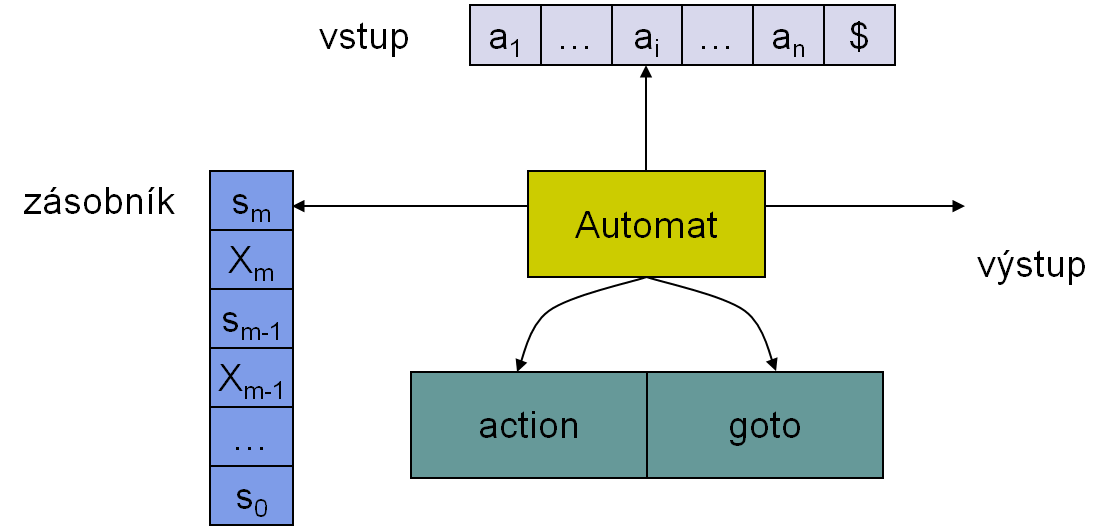
\includegraphics[width=13cm]{i2/softwarove_inzenyrstvi/obrazky/LR_automat.png}
	\caption{LR automat.}
	\label{pic:LR_automat}
\end{figure}

Obrázek \ref{pic:LR_automat} popisuje strukturu LR automatu. V zásobníku jsou zde namíchána čísla stavů (\(s_i\)) a symboly gramatiky (\(X_i\)). Ve skutečné implementaci se však tyto dvě skupiny neukládají do jednoho zásobníku, ale do dvou a místo symbolů gramatiky jsou v zásobníku uloženy podstromy derivačního stromu. A potom je tady ještě tabulka, která obsahuje akce a \uv{goto}. V tabulce akcí (označme \(A\)) se adresuje pomocí stavu (\(s\)) a terminálu (\(a\)) a v buňkách obsahuje instrukce pro další práci automatu. Adresovat v této tabulce budeme tedy pomocí výrazu \(A[s, a]\). V tabulce \uv{goto} (\(G\)) se adresuje pomocí stavu (\(s\)) a neterminálu (\(A\)). V buňkách této tabulky se nachází čísla nových stavů. Adresaci v tabulce \uv{goto} budeme zapisovat jako \(G[s, A]\). Tabulka \uv{goto} se využívá jen u některých instrukcí, jak bude vidět na následujícím popisu funkce automatu.

\paragraph{Funkce LR automatu} Na začátku je hlava nastavena na začátek vstupu a na zásobníku je jen počáteční stav (označme \(s_0\)). V každém kroku se pro vrchol zásobníku \(s_m\) a čtený vstup \(a_i\) provedou následující činnosti:

\begin{penumerate}
	\item Pomocí \(A[s_m, a_i]\) zjistíme instrukci \(I\) a podle jejího typu budeme postupovat dále.
		\begin{penumerate}
			\item \(I\) je typu \emph{shift} s parametrem \(s\). Pak \(a_i\) dám na zásobník, posuneme hlavu o 1 symbol dál a na zásobník dáme \(s\).
			\item \(I\) je typu \emph{reduce} s parametrem \(A \to \alpha\), což je pravidlo gramatiky. Ze zásobníku odstraníme tolik dvojic \((s_k, X_k)\), jak dlouhý je řetězec \(\alpha\) (jednotkou je jeden symbol). Označme \(s\) stav, který zbyl na vrcholu zásobníku. Pomocí \(G[s, A]\) zjistíme stav \(s'\). Na vrchol zásobníku přidáme \(A\) a \(s'\). Na výstup vygenerujeme použití pravidla \(A \to \alpha\).
			\item \(I\) je typu \emph{accept}. Vstupní slovo bylo úspěšně rozpoznáno, máme tedy vygenerovanou derivaci.
			\item \(I\) je typu \emph{error}. Vstupní slovo neodpovídá gramatice.
		\end{penumerate}
\end{penumerate}

Nyní se budeme zabývat tím, jak zkonstruovat LR automat, tedy zejména konstrukcí tabulek. K tomu budeme potřebovat mj. různé podivnosti jako jsou otečkovaná pravidla a kanonické kolekce.

\vskip 1em
\begin{definiceN}{Rozšíření gramatiky}
	Mějme gramatiku \(G = (T, N, S, P)\). \emph{Rozšířením gramatiky} \(G\) je gramatika \(G' = (T, N', S', P')\), kde \(N' = N \cup \{S'\}, P' = P \cup \{S' \to S\}.
\end{definiceN}

Cílem rozšíření gramatiky je pomoci parseru s rozpoznáváním konce parsování. Rozšíření tedy není třeba provádět, pokud už původní gramatika má pouze jedno pravidlo pro počáteční neterminál \(S\) a \(S\) se nevyskytuje na pravé straně žádného z pravidel gramatiky.

\vskip 1em
\begin{definiceN}{Otečkované pravidlo}
	\emph{Otečkované pravidlo} gramatiky \(G\) je pravidlo, které má na pravé straně na nějaké pozici speciální symbol tečky. Speciální znamená, že stejné pravidlo s tečkou na různých pozicích na pravé straně se chápe jako různá otečkovaná pravidla. Zároveň však tato tečka není ani terminálem ani neterminálem gramatiky.
\end{definiceN}

\newcommand{\tecka}{\bullet}

Otečkované pravidlo se také nazývá LR(0) položka. Tečku v pravidle lze chápat jako označení místa, kde se právě parser nachází. Příklad otečkovaného pravidla: \(E \to E + \tecka T\)

\vskip 1em
\begin{definiceN}{Operace uzávěru}
	Mějme množinu otečkovaných pravidel \(I\) z gramatiky \(G = (T, N, S, P)\). Definujme operaci \(CLOSURE(I)\) jako množinu otečkovaných pravidel zkonstruovaných z \(I\) následujícím postupem:
	\begin{penumerate}
		\item Přidej do \(CLOSURE(I)\) množinu \(I\).
		\item \(\forall A \to \alpha \tecka B \beta \in CLOSURE(I)\) (tedy pravidla, kde je tečka těsně před neterminálem), kde \(B \in N\), přidej \(\forall B \to \gamma \in P\) do \(CLOSURE(I)\) otečkované pravidlo \(B \to \tecka \gamma\), pokud tam ještě není. Toto opakuj tak dlouho, dokud přibývají pravidla do \(CLOSURE(I)\).
	\end{penumerate}
\end{definiceN}

Dalo by se přibližně říci, že do \(CLOSURE(I)\) postupně přidáváme pravidla tak, že pokud přidáváme pravidlo \(B\) podle pravidla \(A\), tak tečka v \(B\) je umístěna tak, že pokud by se parser nacházel v místě tečky v pravidle \(A\) a věděli bychom, že se musí použít pravidlo \(B\), tak se v tom samém okamžiku bude parser nacházet v místě tečky v \(B\).

\vskip 1em
\begin{definiceN}{Operace přechodu}
	Definujme operaci \(GOTO(I, X)\) pro množinu otečkovaných pravidel \(I\) a symbol gramatiky \(X\) jako uzávěr množiny všech pravidel \(A \to \alpha X \tecka \beta\) takových, že \(A \to \alpha \tecka X \beta \in I\).
\end{definiceN}

Definice vlastně říká, že chceme-li udělat množinu \(GOTO(I, X)\), musíme z \(I\) vzít všechna otečkovaná pravidla, ve kterých je tečka těsně před symbolem \(X\). Potom v těchto pravidlech tečku posunout těsně za symbol \(X\) a udělat uzávěr z této množiny.

\paragraph{Konstrukce KKMOP} Kanonickou kolekci množin otečkovaných pravidel vytvoříme takto: Mějme rozšířenou gramatiku \(G' = (T, N', S', P')\). Budeme konstruovat kolekci \(C\). Na počátku položíme \(C = \{ CLOSURE(\{S' \to \tecka S\})\}\). Následně \(\forall I \in C a \forall X \in T \cup N'\) takové, že \(GOTO(I, X) \notin C \wedge GOTO(I, X) \neq \emptyset\), přidej \(GOTO(I, X)\) do \(C\). Toto opakujeme dokud něco přibývá do \(C\).

Je potřeba si uvědomit, že \(C\) je množina množin, takže na začátku obsahuje jen jeden prvek, tedy množinu \(CLOSURE(\{S' \to \tecka S\})\). Na příklad takové konstrukce se raději podívejte na slajdy p. Yaghoba k Principům překladačů, kde je vidět jak konstrukce postupně probíhá.




\subsection{Syntaxí řízený překlad a atributové gramatiky.}
\subsection{Reprezentace programu mezikódem.}
\subsection{Překlad výrazů a programových struktur.}
\subsection{Rozsahy platnosti proměnných, aktivační záznamy, implementace vnořených procedur, volací konvence.}
\subsection{Vliv architektury počítače na generování kódu a optimalizaci.}
\subsection{Metody generování kódu, přidělování registrů, scheduling, optimalizace.}
\subsection{Podpora kompilátorů pro synchronizační primitiva, vlákna.}
\subsection{Objektově orientované jazyky a principy jejich implementace.}
\subsection{Překladače vs. interpretry, skriptovací jazyky.}

\input{i2/softwarove_inzenyrstvi/Objektove_orientovane_a_komponentove_systemy.tex}
\input{i2/softwarove_inzenyrstvi/Analyza_a_navrh_softwarovych_systemu.tex}


\end{document}